\setcounter{subsection}{0}
\section{RESULTADOS}

El capítulo anterior describió cómo se construyó cada etapa y qué se descartó en el camino. Este
capítulo responde si lo construido funciona, objetivo por objetivo, y encontró que la lectura de las listas, la decisión de
aceptar un renglón sin revisión y el armado de kits cumplen con medidas propias, y que los acudientes
completaron la compra. Es la etapa de evaluación de CRISP-DM para los componentes que dependen de datos
(OE3 y OE4, fases F3 y F4 de la Tabla~\ref{tab:fases}), complementada con el control de calidad por
características de la ISO/IEC 25010 y con la evaluación con usuarios, que siguió un protocolo
preregistrado (OE5, fase F5). Cada objetivo se presenta con el mismo esquema: la pregunta, el método y la
etapa en que se ubica, la métrica, los datos, el resultado con su incertidumbre y su punto de
comparación, la lectura y el límite. Cada cifra va con su muestra y su condición, y cuando dos fuentes
discrepan o falta el programa que produjo un valor, el texto lo dice en lugar de darlo.

La Tabla~\ref{tab:metricas} resume el capítulo antes de entrar al detalle.

\begin{table}[htbp]
\centering
\caption{Resumen de resultados por objetivo}
\label{tab:metricas}
\footnotesize
\begin{tabularx}{\linewidth}{@{}p{1.5cm}p{3.0cm}p{3.2cm}Xl@{}}
\toprule
\textbf{Objetivo} & \textbf{Pregunta} & \textbf{Métrica} & \textbf{Resultado} & \textbf{Estado} \\
\midrule
OE3, lectura & ¿Se recuperan los renglones de una lista sin estructura? & F1 micro y macro & 0,948 y 0,944 (Gemini), frente a 0,298 de las reglas & Cumplido \\
OE3, decisión & ¿Lo que se acepta sin revisión es correcto? & Precisión y cobertura en $\tau = 0{,}75$ & \calTauP{} (IC 95\,\% \calTauPBajo--\calTauPAlto) con \calTauAceptada{} aceptado & Cumplido \\
OE4 & ¿Los kits quedan cerca del frente óptimo y a tiempo? & Razón de hipervolumen; p95 de tiempo & 0,9969; 0,31~s (límite 8~s) & Cumplido \\
OE5 & ¿Funciona el sistema integrado y lo usa un acudiente sin ayuda? & Pruebas, ISO/IEC 25010, éxito sin ayuda, SUS & 2.542 pruebas; 6 de 6 pagaron; SUS 90 [82--98] & Cumplido \\
\bottomrule
\end{tabularx}
\end{table}

% =====================================================================
\subsection{Percepción documental}
\label{sec:percepcion}

\textbf{Pregunta.} El primer criterio del árbol de utilidad exige extraer de una lista escolar,
entregada como imagen o PDF sin estructura, los renglones con su cantidad y su descripción.
\textbf{Método.} Es la etapa de evaluación de CRISP-DM aplicada a la comparación de cinco motores que
hicieron los prototipos de tesis el 1 de septiembre de 2026. \textbf{Métrica.} El $F_1 = 2PR/(P+R)$ mide si
la lectura recupera los renglones correctos sin inventar otros; el micro suma los aciertos de todos los
renglones y el macro promedia el $F_1$ por documento, de modo que un documento largo no tape a uno
corto. Un renglón acierta si su similitud con el del oro es de al menos 0,75. \textbf{Datos.} CGS-10, un
conjunto de oro de diez documentos y 1.293 ítems, armado corrigiendo la extracción de uno de los
motores, sin un segundo anotador.

\textbf{Resultado.} La Tabla~\ref{tab:percepcion} ordena los motores por $F_1$; los valores se
recalcularon desde la salida conservada, sin volver a ejecutarlos. El modelo multimodal de Gemini
llegó a 0,948 y 0,944, frente a 0,673 de Google Vision y 0,298 de las reglas heurísticas, que es el
punto de comparación más simple. El acta del OE3 consigna 0,925, un valor que no proviene de esa
salida y que por eso no se usa.

\begin{table}[htbp]
\centering
\caption{Percepción documental en los prototipos de tesis (CGS-10, diez documentos)}
\label{tab:percepcion}
\small
\begin{tabular}{@{}lrr@{}}
\toprule
\textbf{Enfoque} & \textbf{F1 micro} & \textbf{F1 macro} \\
\midrule
Gemini (multimodal) & 0,948 & 0,944 \\
Google Vision & 0,673 & 0,672 \\
GOT-OCR2.0 & 0,597 & 0,569 \\
Docling & 0,364 & 0,424 \\
OCR con reglas heurísticas & 0,298 & 0,419 \\
\bottomrule
\end{tabular}
\end{table}

\textbf{Lectura.} La ventaja del modelo multimodal sobre las reglas es amplia y justifica haberlo
elegido. \textbf{Límite.} El oro coincide con la salida de Gemini en el 86,7\,\% de los ítems literales y
en el 93,1\,\% sin tildes ni puntuación, así que el 0,948 no es independiente de ese motor y su
magnitud está sesgada a su favor. Además, son diez documentos con una sola corrida por motor, y el
sistema construido usa otro modelo de Gemini, con temperatura 0 y sin semilla. La latencia de la
percepción con el modelo real se mide en el segundo nivel de las pruebas (ESC-D1 del ATAM), porque la
verificación del primer nivel usó una percepción
simulada\pendienteEvidencia{latencia de la percepcion con el modelo real, DP-04}.

% =====================================================================
\subsection{Recuperación y decisión de resolución}
\label{sec:recuperacion}

\textbf{Pregunta.} Una vez leído un renglón, ¿el sistema encuentra su concepto canónico y decide
bien cuándo aceptarlo sin revisión? \textbf{Método.} También es la etapa de evaluación de CRISP-DM
del OE3, con cuatro mediciones: la recuperación de candidatos, el acuerdo en la clasificación del
corpus, la decisión con el umbral $\tau$ y el recorrido de extremo a extremo.
\textbf{Métrica.} MRR@10, $\frac{1}{|Q|}\sum_q 1/r_q$, con $r_q$ el rango del primer acierto entre 10,
que importa porque el sistema muestra pocos candidatos; kappa de Cohen, $\kappa=(p_o-p_e)/(1-p_e)$, que
descuenta el acuerdo por azar; y, para la decisión, la precisión (de lo aceptado, cuánto era correcto),
la cobertura (qué fracción se acepta sin revisión) y el AUC de la curva ROC.

\textbf{Datos.} Los prototipos compararon cuatro estrategias sobre PostgreSQL con pgvector (léxica
pura, léxica expandida, vectorial densa e híbrida con fusión recíproca de rangos), y el sistema
construido adoptó la fusión aditiva de una sola fase (Sección~\ref{sec:normalizacion}). El kappa
usa 200 pares de 12 documentos. La decisión con $\tau$ usa \calTauPares{} pares renglón-concepto de
\calTauListas{} listas de \calTauColegios{} colegios, que un revisor marcó como correctos o incorrectos;
la corrida se hizo el 5 de noviembre sobre la versión evaluada \texttt{b6b6fe7}.

\textbf{Resultado: recuperación.} La léxica pura tuvo un p50 de 6,66\,ms; la vectorial densa, de
46,51\,ms, y la híbrida, de 53,17\,ms; la medición registra tiempo y no relevancia. En la tarea
SpanishPassageRetrievalS2P de MTEB \citep{muennighoff_mteb_2023}, de pasajes de salud y no escolares,
multilingual-e5-large obtuvo un MRR@10 de 0,6163 frente a 0,4735 de paraphrase-multilingual-mpnet-base-v2.
El sistema construido calcula hoy los embeddings con gemini-embedding-001, así que esta cifra solo
respalda la elección del modelo de los prototipos. Sobre Recall@10 hay una discrepancia sin resolver:
un informe reporta 1,0000 y la única salida conservada da 0,10 para los índices aproximados, sin el
programa que la produjo, por lo que no se afirma ningún valor. La latencia de la recuperación del
sistema construido tampoco se midió
\pendienteEvidencia{latencia de la recuperacion de candidatos en el sistema construido}.

\textbf{Resultado: acuerdo en el corpus.} El kappa fue de 0,7331, con intervalo del 95\,\% por
remuestreo de [0,670; 0,794], y se reprodujo desde las entradas conservadas. Compara la categoría que
asigna una heurística con la de un modelo de lenguaje en 45 de las 48 categorías, de modo que describe la
concordancia entre dos métodos automáticos y no entre dos personas. La meta del SPMP (IEEE 1058) exige
$\kappa \ge 0{,}7$ con un segundo anotador humano sobre al menos 30 documentos; esa medición está en
organización\pendienteEvidencia{kappa entre dos anotadores humanos ciegos, n>=30 documentos}.

\textbf{Resultado: decisión con $\tau$.} El sistema acepta un renglón sin revisión cuando su puntaje
de similitud llega a $\tau = 0{,}75$ y lo envía a revisión en otro caso. La
Figura~\ref{fig:tau-clasificacion} muestra a la izquierda cuántos de los \calTauPares{} pares acertó
esa regla, en el centro cómo cambian la precisión y la cobertura al mover $\tau$ y a la derecha la
curva ROC; el punto naranja marca $\tau = 0{,}75$.

\begin{figure}[htbp]
\centering
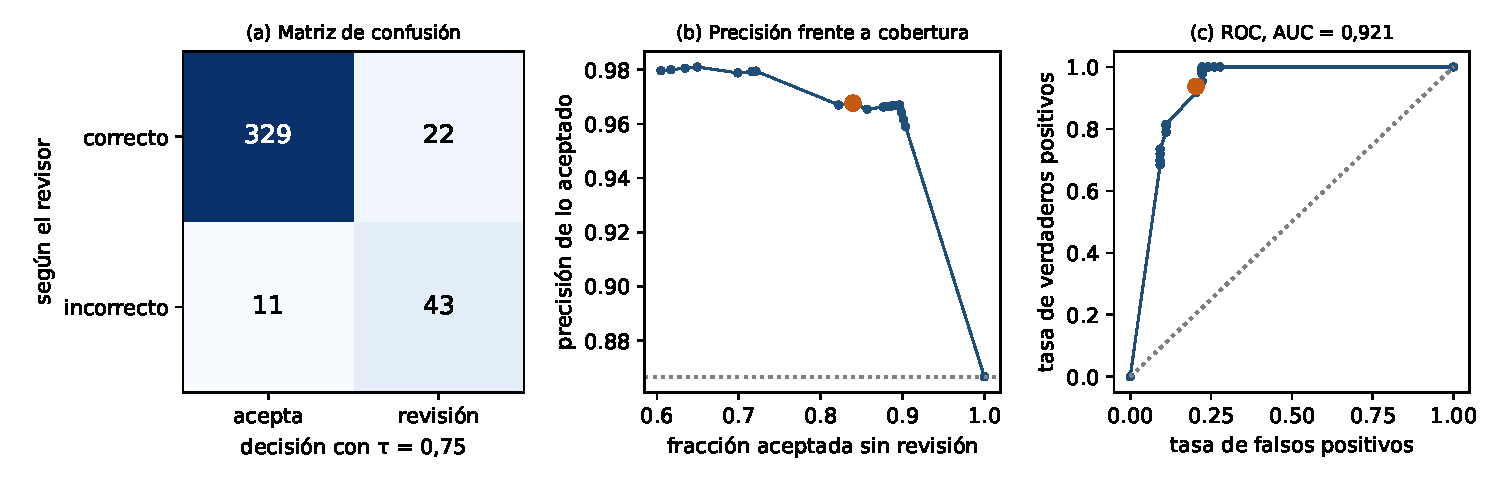
\includegraphics[width=\linewidth]{tau_clasificacion.pdf}
\caption{Decisión de aceptar o revisar con $\tau = 0{,}75$ sobre \calTauPares{} pares: (a) matriz de
confusión, (b) precisión frente a cobertura, (c) curva ROC. La línea punteada de (b) es la precisión de
aceptar todo.}
\label{fig:tau-clasificacion}
\end{figure}

En $\tau = 0{,}75$ se aceptaron \calTauTP{} pares correctos y \calTauFP{} incorrectos, y se enviaron a
revisión \calTauFN{} correctos y \calTauTN{} incorrectos. La precisión fue de \calTauP{} (IC 95\,\% por
\emph{bootstrap} de \calTauPBajo{} a \calTauPAlto{}), la sensibilidad de \calTauR{}
(\calTauRBajo{}--\calTauRAlto{}), el $F_1$ de \calTauF{} (\calTauFBajo{}--\calTauFAlto{}) y la cobertura
de \calTauAceptada{}. En palabras llanas: de cada 100 renglones aceptados sin revisión, 97 eran
correctos, y el sistema se ahorró la revisión de cuatro de cada cinco. Aceptar todo daría una
precisión de 0,867, el punto de comparación (\calTauAciertos{} aciertos de 405). El AUC fue de
\calTauAUC{} (\calTauAUCBajo{}--\calTauAUCAlto{}). Se destaca la precisión frente a la cobertura y no la
ROC porque las clases están desbalanceadas, 351 correctos contra 54 incorrectos, y en ese caso la
ROC se ve mejor de lo que es \citep{saito_precision-recall_2015}. Una validación cruzada agrupada
indica que bastaría un $\tau$ entre \calTauCVMin{} y \calTauCVMax{} para llegar a 95\,\% de precisión;
por eso 0,75 es más conservador de lo necesario y manda a revisión más renglones de los que haría
falta. El AUC de 0,961 de una corrida anterior bajó a \calTauAUC{} porque los datos se volvieron a
correr sobre la versión evaluada \texttt{b6b6fe7} después de la curaduría de noviembre.

\textbf{Resultado: extremo a extremo.} El 83\,\% de una corrida anterior (60 sublistas, 2.176 ítems)
mide la fracción de ítems con algún candidato (83,04\,\%), no la resolución: 35,3\,\% se resolvió de
forma automática, 36,5\,\% pasó a revisión y 28,1\,\% quedó sin correspondencia. Un ensayo de huecos
del 21 al 23 de septiembre aplicó las primeras versiones del sistema a 14 PDF (4.414 renglones): se
reconocieron 2.202, 926 terminaron en abstención (20,98\,\%) y quedaron 1.397 faltantes únicos para la
curaduría del catálogo.

\textbf{Lectura.} La regla de decisión es confiable en lo que acepta y prudente en lo que deja pasar a
revisión, que es el error más barato. \textbf{Límite.} Un solo revisor etiquetó los pares y no hay
acuerdo entre personas. El puntaje toma solo \calTauValores{} valores distintos, de modo que $\tau$ no
se puede afinar y las curvas avanzan a saltos. Son tres colegios, y las latencias y el extremo a
extremo vienen de prototipos y de un espejo de 838 productos que el sistema construido ya no usa.

% =====================================================================
\subsection{Optimización}
\label{sec:optimizacion}

\textbf{Pregunta.} ¿Los kits que arma el optimizador quedan cerca del frente óptimo y a tiempo?
\textbf{Método.} Es la etapa de evaluación de CRISP-DM del OE4, con el escenario ESC-D4 del ATAM
(OE2) como prueba de tiempo. \textbf{Métrica.} La razón de hipervolumen
\citep{zitzler_multiobjective_1999}, $HV(\text{frente})/HV(\text{exacto})$ con punto de referencia común
de 1,1 por eje normalizado, mide cuánto del frente óptimo conserva NSGA-II sin necesitar un kit de
referencia único; el p95 de tiempo, la demora del 5\,\% más lento, que el promedio esconde.
\textbf{Datos.} Las 175 instancias del banco, de 174 listas de 17 colegios, de las cuales 40 forman el
conjunto de prueba que se apartó por colegio y se usó una vez (Sección~\ref{sec:optimizacion-cal}).

\textbf{Resultado.} En las 32 listas de prueba resueltas con NSGA-II (las otras 8 se resolvieron de
forma exacta), el frente alcanzó en promedio 0,9969 del hipervolumen exacto. Contra un óptimo por
programación dinámica en 174 listas, NSGA-II lo iguala en el 100\,\% de las listas del Ahorrador; con
presupuesto, el kit recomendado daba el 40\,\% de la calidad posible y, después del ADR 0029, cabe
siempre en el tope e iguala el óptimo (una semilla, cifra reportada). El banco de alternativas del 31
de julio, de nueve instancias sintéticas con tres objetivos, dio una referencia: NSGA-II halló el
óptimo en ocho y quedó a 0,07\,\% de él, frente a 11,92\,\% del voraz y 159,34\,\% del aleatorio. Para
el tiempo se corrió ESC-D4 con las 175 instancias, 30 ejecuciones por lista con semillas distintas y dos
perfiles de acudiente, 10.500 ejecuciones en un Apple M4: el p95 fue de 0,29~s sin preferencias y de
0,31~s con personaje, el máximo de 0,45~s, frente a los 8~s de DP-03, un margen de más de 25 veces. En
el banco de Tukit-Benchmarks, que midió el mismo optimizador, la programación dinámica equivalió a la
enumeración en 65 de 65 listas y fue más rápida en las listas reales (mediana de 0,64~ms frente a
243~ms), pero con un hogar de ocho hijos y 313 líneas tardó 2,56~s y 297~MiB, contra 1,46~s y 12,6~MiB
de NSGA-II.

Más allá del optimizador, se auditaron cuatro veces, renglón por renglón, los kits Ahorrador y Premium de
las trece listas de 2026 del Colegio Agustiniano Ciudad Salitre, el 11 y el 12 de octubre. Un renglón cumple
si los dos perfiles cobran lo que pide la lista. La Tabla~\ref{tab:kits} muestra que el cumplimiento
subió en cada auditoría, de 29,6\,\% a 85,6\,\%, mientras se ajustaban la comparación de atributos y la
curaduría y el catálogo pasaba de 679 a 1.030 productos con precio. Los cobros de un producto que no
corresponde bajaron de 589 a 49 y subieron a 58 en la cuarta, por 23 cuadernos que no dicen ser grandes. De
los 69 huecos finales, 45 son de electrónica, que las tiendas registradas no ofrecen.

\begin{table}[htbp]
\centering
\caption[Auditorías de los kits del Colegio Agustiniano Ciudad Salitre]{Auditorías de los kits del Colegio Agustiniano Ciudad Salitre, 11 y 12 de octubre de
2026; las dos últimas, posteriores a la versión evaluada (cifras reportadas; costo de los trece kits de cada perfil)}
\label{tab:kits}
\small
\begin{tabular}{@{}lrrrrr@{}}
\toprule
\textbf{Auditoría} & \textbf{Comprables} & \textbf{Huecos} & \textbf{Cobros} &
\multicolumn{2}{c}{\textbf{Costo (millones de pesos)}} \\
\cmidrule(l){5-6}
 & \textbf{que cumplen} & \textbf{declarados} & \textbf{sin cumplir} & \textbf{Ahorrador} &
\textbf{Premium} \\
\midrule
1 (11 oct.) & 263 de 888 (29,6\,\%) & 240 & 589 & 13,9 & 32,0 \\
2 (11 oct.) & 465 de 888 (52,4\,\%) & 385 & 242 & 9,9 & 17,6 \\
3 (11 oct.) & 617 de 886 (69,6\,\%) & 220 & 49 & 9,0 & 14,2 \\
4 (12 oct.) & 758 de 885 (85,6\,\%) & 69 & 58 & 8,1 & 17,3 \\
\bottomrule
\end{tabular}
\end{table}

\textbf{Lectura.} El frente de producción conserva casi todo el hipervolumen exacto con una fracción
del tiempo permitido, y el cumplimiento de los kits mejora con cada ajuste del catálogo y de las
reglas. \textbf{Límite.} Las cifras del banco de julio y de la programación dinámica son
reportadas, con una sola semilla, y la resolución de las listas usó solo el canal léxico y una foto
fija del catálogo. La medición de tiempo cubre la optimización, no la lectura ni la recuperación. Las
auditorías cubren un colegio, dependen de una clasificación humana y midieron versiones intermedias,
no el sistema construido.

% =====================================================================
\subsection{Verificación del sistema integrado}
\label{sec:calidad}
\label{sec:calidad-resumen}
\label{sec:control-calidad}
\label{sec:defectos}

\textbf{Pregunta.} Con cada etapa evaluada por separado, ¿el sistema ya integrado funciona, resiste
carga y protege los datos de quien lo usa?

\textbf{Método.} Es la parte de pruebas del OE5 (fase F5). El equipo de calidad ejecutó un plan de diez
fases, ordenado por las características del modelo de calidad ISO/IEC 25010 \citep{iso_25010_2011}: 0 línea
base, 1 escenarios de requisitos no funcionales, 2 unitarias y cobertura, 3 integración, 4 funcionales,
5 adversariales de IA, 6 patrones de resiliencia, 7 caos, 8 carga y 9 telemetría. Las fases 0 a 6 se corrieron
en octubre y la campaña de caos, carga y telemetría llegó hasta el 5 de noviembre de 2026.

\textbf{Métrica.} Pruebas aprobadas, cobertura de sentencias, tiempo de recuperación, errores y percentil 95 de
latencia bajo carga, y hallazgos por severidad. \textbf{Datos.} Los de cada nivel, resumidos en la
Tabla~\ref{tab:niveles-prueba}, más dos auditorías de código: la de autorización (152 puntos de entrada) y la
de datos personales conforme a la Ley 1581 de 2012 \citep{congreso_ley1581_2012}.

\begin{table}[htbp]
\centering
\small
\caption{Niveles de prueba del sistema integrado.}
\label{tab:niveles-prueba}
\begin{tabularx}{\textwidth}{@{}p{2.3cm}XXX@{}}
\toprule
Nivel & Qué verifica & Datos & Resultado \\
\midrule
Unitarias y cobertura & Bibliotecas y servicios, con los defectos conocidos marcados como fallo esperado & 2.542 pruebas Python, 86 de la web y 67 de contrato & Todas pasan; cobertura de 54\,\% (catálogo) a 98\,\% (puerta de enlace) \\
Integración & Los servicios contra el sistema desplegado completo & Bases de prueba aisladas y fronteras entre servicios & Pasan; la prueba de humo pasó \\
Funcionales & Percepción y emparejamiento con conjuntos de oro & G01-G10, lista base de 18 renglones; el oro fija la respuesta del modelo y mide al sistema & 0 productos fuera del catálogo \\
Adversariales de IA & OWASP LLM 2025 & 143 pruebas & 120 verdes; inyección en texto e imagen y producto inexistente cumplen \\
Resiliencia y caos & Caídas inyectadas con Toxiproxy & Campaña del 5 de noviembre: 25 ensayos & 14 cumplen \\
Carga & Rampa de 5 a 100 usuarios (L-02) & Apple M4 y Windows con WSL2 & 0 errores en el M4; saturación en WSL2 \\
Telemetría & Expedientes por identificador de correlación & Trazas de 2 expedientes (32 tramos) & No cumple \\
Seguridad & Pago sin datos de tarjeta; autorización & Barrido de 248 columnas & 0 números de tarjeta \\
\bottomrule
\end{tabularx}
\end{table}

\textbf{Resultado: pruebas automáticas.} De las 2.542 pruebas Python ninguna falló y una quedó saltada
(la prueba en vivo del asistente, que necesita la llave del modelo). La integración continua no exige un
mínimo de cobertura, así que esta describe el estado y no una meta.

\textbf{Resultado: adversariales de IA.} De 143 pruebas, 23 documentan un defecto. Dejaron hallazgos el
esquema roto (cuatro formas devolvían error 500 en lugar de 422), la fuga del prompt, los datos personales, la
agencia excesiva, los embeddings, el consumo sin tope y los identificadores de correlación hostiles.

\textbf{Resultado: requisitos no funcionales.} La matriz tiene 52 requisitos en 99 filas: 54 ejecutadas,
25 por medir, 9 omitidas y 8 no medibles. 

\textbf{Resultado: degradación.} Con el catálogo colgado, el disyuntor abre a los 26,3~s, dentro de los 30~s
de ESC-R2. La campaña del 5 de noviembre dio 26,4 y 26,3~s.

\textbf{Resultado: caídas.} En la campaña de octubre fallaron tres escenarios; su corrección se verificó en una rama aparte, que la versión evaluada no integra. En CH-04, con el catálogo caído,
la subida de la lista devolvía error 500 y no se guardaba. En CH-12 y CH-15, con PostgreSQL o RabbitMQ caídos,
los procesos de fondo no volvían, y un pago avisaba dos veces. Tras la corrección (verificación del 20 de
octubre), la subida responde 202 en 33~ms y se recupera en 2,7~s, CH-12 en 7,1~s, CH-15 en 6,9~s, y el pago manda un solo aviso.

\textbf{Resultado: carga.} El requisito RNF05 (decisión de diseño DP-02) pide 50 usuarios con menos de
5\,\% de error. En un Apple M4 con los servicios nativos (5 de noviembre), la rampa completó 25.706 peticiones
sin un error y sin saturación hasta 100 usuarios; el percentil 95 del catálogo (la demora que no supera el
95\,\% de las peticiones) fue de 49 a 420~ms hasta 50 usuarios y de 2,5~s con 100. En Windows con WSL2 y
4 CPU, el catálogo se saturó desde 30 usuarios, con un núcleo al 100\,\%. Por eso RNF05 se cumple en el M4,
con el doble de usuarios pedido. El umbral adicional de 300~ms para el percentil 95 se supera desde 25 usuarios
porque el catálogo corre en un solo proceso (Sección~\ref{sec:trabajo-futuro}).

\textbf{Resultado: seguridad.} La auditoría de dependencias de la web quedó en cero vulnerabilidades. Si
alguien pide el kit de otra persona, el sistema responde con error 401 (no autenticado) cuando no hay
sesión y con error 404 (no existe) cuando la sesión es de otra cuenta. La auditoría de autorización halló
22 de 152 puntos de entrada que no comparaban por completo a qué cuenta pertenece cada dato, y de seis
hallazgos de esa revisión se cerraron cuatro. El defecto de mayor alcance, las políticas de acceso a nivel
de fila de la base de datos que concedían la tabla completa, se evita porque el sistema controla ese acceso
en la aplicación (Sección~\ref{sec:autorizacion}).

\textbf{Resultado: hallazgos de calidad.} El registro del control de calidad cuenta 85 hallazgos vigentes del sistema evaluado
al 5 de noviembre (16 de severidad alta, 58 media y 11 baja) y 10 cerrados. Los defectos de código tienen además una prueba que se espera
que falle (\texttt{xfail} estricto): si el defecto se corrige y la prueba pasa, la prueba falla y obliga
a cerrar el hallazgo. Entre los de severidad alta están las rutas de administración sin sesión, el
administrador sin segundo factor de autenticación y el nombre del menor, que llega sin depurar al
proveedor del modelo.

El recorrido completo se evalúa así. Con pago simulado, dos corridas
automáticas dieron resultados distintos: el pedido llegó a «pagado» el 1 de noviembre y quedó «pendiente
de pago» el 2, por un fallo de la consulta de estado que no se repitió. En cambio, en las seis sesiones
con acudientes el pedido terminó pagado. Con eso se da por funcional el recorrido hasta el pago simulado.

La Tabla~\ref{tab:iso25010} ordena la evidencia por característica de la ISO/IEC 25010 («Parcial»: falta
alguna prueba o hay hallazgos abiertos). T4, T6 y C3 se definen en la Sección~\ref{sec:oe5}.

\begin{table}[htbp]
\centering
\scriptsize
\caption{Evidencia de calidad por característica de la ISO/IEC 25010.}
\label{tab:iso25010}
\begin{tabularx}{\textwidth}{@{}lXl@{}}
\toprule
Característica & Evidencia & Estado \\
\midrule
Adecuación funcional & 2.542 pruebas Python y las de las dos aplicaciones web; recorrido de la cuenta al pago con acudientes; personaje del segundo hijo sin reflejar en el kit Fan & Parcial \\
Eficiencia de desempeño & ESC-D4 con p95 de 0,31~s frente a 8~s; L-02 hasta 100 usuarios sin errores en el M4, con p95 del catálogo de 49 a 420~ms hasta 50 usuarios, y saturación desde 30 en la máquina virtual & Parcial \\
Compatibilidad & Pruebas de fronteras entre servicios (75) y del contrato entre la web y la API (67) & Probada \\
Usabilidad & Seis sesiones con acudientes: T6 4 de 5 y T4 1 de 5 sin ayuda; SUS medio de 90 [82--98]; C3 solo en T6 & Parcial \\
Fiabilidad & Campaña de caos del 5 de noviembre (14 de 25 ensayos cumplidos); hallazgos de idempotencia y avisos abiertos & Parcial \\
Seguridad & Lectura de kits ajenos cerrada, 0 vulnerabilidades web, 0 de 81 ataques al asistente; un token en el historial; hallazgos de severidad alta abiertos & Parcial \\
Mantenibilidad & Cobertura de 54 a 98\,\% por servicio, sin umbral en la integración continua & Parcial \\
Portabilidad & Infraestructura con Docker Compose y servicios locales con el sistema desplegado completo; sin pruebas en dispositivos & Parcial \\
\bottomrule
\end{tabularx}
\end{table}

\textbf{Lectura.} El sistema integrado cumple la capacidad pedida y el recorrido hasta el pago simulado
funciona; sin embargo, solo una de las ocho características de la ISO/IEC 25010 quedó probada por
completo. Los hallazgos de seguridad y privacidad deben cerrarse antes de operar con datos y pagos
reales, y por eso encabezan el trabajo futuro.

\subsection{Evaluación con usuarios}
\label{sec:oe5}

\textbf{Pregunta.} Las pruebas automáticas de la sección anterior verifican el código, pero no muestran si
un acudiente, sin que nadie le explique la aplicación, logra armar y pagar el kit de su hijo. Esta
evaluación lo responde. \textbf{Método.} Es la fase F5 del OE5, con un protocolo
preregistrado: el plan de análisis, con tareas, métricas y criterios de éxito, se fechó el 28 de octubre de
2026, antes de la primera sesión, para no ajustar los criterios
a los resultados. Cada sesión fue una prueba de usabilidad moderada con pensamiento en voz alta
\citep{lazar_research_2017}, sin instrucciones. Las tareas siguen la compra: crear la cuenta y elegir colegio
y grado (T1), declarar personaje y gasto (T2), esperar la generación (T3), revisar y elegir un kit (T4),
cambiar o quitar un producto (T5), pagar (T6) y encontrar el pedido (T7); T8, pedir un cambio al asistente,
es exploratoria y no se planteó a los participantes. T1, T4 y T6 son críticas.

\textbf{Métrica.} Cada tarea se codificó como éxito sin ayuda, con ayuda, fallo o falla del sistema, con
criterio estricto: cualquier indicación de la moderadora cuenta como ayuda. Además se definieron tres
criterios. C1: el SUS (System Usability Scale, cuestionario de diez preguntas con puntaje de 0 a 100) debe
superar 68, el valor medio de referencia. C2: la carga percibida, medida con el RTLX (Raw Task Load Index, de
0 a 100, donde más es más carga), debe ser menor con Tukit que en la última compra habitual, con un intervalo
que excluya el cero y un tamaño del efecto $d_z \ge 0{,}5$. C3: cada tarea crítica debe lograrse sin ayuda en
al menos 80\,\% de las sesiones. También se aplicó el NPS (Net Promoter Score, cuánto recomendarían la
aplicación), que se reporta sin criterio.

\textbf{Datos.} Participaron seis acudientes del Colegio Agustiniano Ciudad Salitre, el colegio piloto,
reclutados por conveniencia entre el 2 y el 3 de noviembre (cinco por videollamada, uno presencial). El pago
usó la pasarela en modo simulado. La primera sesión de ACU-04 se cortó al subir la lista, así que de ella
solo se codifica T1; su segunda grabación muestra el pago aprobado, y por eso se cuentan los seis pagos,
aunque T6 se codifica sobre cinco sesiones. Las sesiones se grabaron con consentimiento, se transcribieron
en el equipo del proyecto y un segundo codificador revisó cada hoja contra las mismas fuentes y dejó 78
correcciones que se incorporaron antes del análisis.

\textbf{Resultado.} La Tabla~\ref{tab:oe5-tareas} da el éxito sin ayuda por tarea con su intervalo de
Wilson. Los seis acudientes completaron el recorrido
de la cuenta a un pedido pagado; el pago (T6) se resolvió sin ayuda en cuatro de cinco sesiones, en una
mediana de 43 segundos, y el registro (T1) en cuatro de seis. El resultado que cambia el diseño es T4: solo
uno de cinco revisó los kits y eligió sin ayuda. Se repitieron tres problemas. Primero, dos acudientes no
encontraron el camino a «Ver mis kits» al terminar la espera. Segundo, no entendieron de dónde sale el kit
(«yo no sé cuánto vale en el Faro», el comercio con el que esa acudiente compara precios) ni qué significa «confiable». Tercero, las listas de 82 productos les
generaron «estrés visual». Hubo además dos fallas puntuales: el asistente flotante tapó el botón «Elegir» y el kit Fan mostró solo el personaje de la primera de dos hijas. Ningún acudiente
usó el asistente por su cuenta.

\begin{table}[htbp]
\centering
\small
\caption{Éxito sin ayuda por tarea en las sesiones con acudientes (n = 6; ACU-04 solo en T1).
Intervalo de Wilson del 95\,\% y mediana del tiempo de la tarea; en T3, la duración de la espera.}
\label{tab:oe5-tareas}
\begin{tabular}{@{}llccc@{}}
\toprule
Tarea & Qué pide & Sin ayuda & IC 95\,\% & Mediana (s) \\
\midrule
T1 (crítica) & Cuenta, colegio y grado & 4 de 6 (67\,\%) & 30--90\,\% & 70 \\
T2 & Personaje y opción de gasto & 3 de 5 (60\,\%) & 23--88\,\% & 32 \\
T3 & Esperar los kits & 4 de 5 (80\,\%) & 38--96\,\% & 50 \\
T4 (crítica) & Revisar los kits y elegir & 1 de 5 (20\,\%) & 4--62\,\% & 91 \\
T5 & Cambiar o quitar un producto & 3 de 5 (60\,\%) & 23--88\,\% & 84 \\
T6 (crítica) & Pagar (simulado) & 4 de 5 (80\,\%) & 38--96\,\% & 43 \\
T7 & Encontrar el pedido & 2 de 2 (100\,\%) & 34--100\,\% & 16 \\
\bottomrule
\end{tabular}
\end{table}

Los cuestionarios, que los seis respondieron el 5 de noviembre, resumen la valoración
(Tabla~\ref{tab:oe5-cuestionario}). El límite inferior del intervalo del SUS supera el umbral de 68 (prueba t
de una muestra, $p = 0{,}0004$) y en la escala de Bangor et al.~\citep{bangor_determining_2009} el promedio
corresponde a «excelente», un valor que orienta y no estima la población. La carga percibida con Tukit fue
mucho menor que la de la última compra habitual, con un intervalo de la diferencia que excluye el cero (prueba
t pareada, $p = 0{,}003$; $d_z$ es la diferencia media dividida por la desviación estándar de las
diferencias). Cuatro de seis describieron la aplicación como fácil, intuitiva o rápida («fue súper rápido»,
ACU-05), y valoraron el ahorro de tiempo y poder cambiar productos. El tiempo activo de las sesiones completas fue de 2,4 a 10,3 minutos, frente a cuatro horas o más
que reporta el 65\,\% de los acudientes en la encuesta del OE1; es solo un orden de magnitud, porque compara
una tarea guiada con una compra real.

\begin{table}[htbp]
\centering
\small
\caption{Cuestionario de cierre (n = 6). SUS y RTLX de 0 a 100; intervalos del 95\,\%
($t$ para SUS y la diferencia de RTLX, \emph{bootstrap} de 10.000 remuestreos para el NPS).}
\label{tab:oe5-cuestionario}
\begin{tabular}{@{}llcc@{}}
\toprule
Medida & Resultado & IC 95\,\% & Criterio \\
\midrule
SUS (C1) & 90 (de 77,5 a 100) & 82--98 & $> 68$: cumple \\
RTLX, compra habitual & 63 & & \\
RTLX, con Tukit & 9 & & \\
Diferencia RTLX (C2) & 54, $d_z = 1{,}83$ & 23--85 & excluye 0 y $d_z \ge 0{,}5$: cumple \\
NPS (S1) & $+83$ (5 promotores, 1 pasivo) & 50--100 & se reporta \\
\bottomrule
\end{tabular}
\end{table}

\textbf{Lectura.} El OE5 pide pruebas funcionales, no funcionales, de carga y de usabilidad con usuarios
reales. Las cuatro clases se ejecutaron, aunque las de carga y degradación quedaron en una corrida por equipo
y sin repetir todos los niveles (Sección~\ref{sec:calidad}). C1 y C2 se cumplen y C3 se alcanzó en el pago (T6),
pero no en el registro (T1) ni en la elección del kit (T4). Con seis participantes los resultados son
formativos \citep{nielsen_estimating_1994}, es decir, sirven para ver dónde se concentra la ayuda y orientar
la siguiente versión. Los primeros cambios apuntan a T4: llevar al acudiente a sus kits cuando estén listos, agrupar los productos por categoría con la tienda
visible, explicar las etiquetas de nivel y los textos de consolidación, corregir el personaje del segundo
hijo, reubicar el asistente y aclarar que la cuenta se crea al armar el kit.

\textbf{Límite.} El plan se desvió en varios puntos. El reclutamiento fue por conveniencia, con una sola ronda y una sola moderadora, y varios participantes conocen al equipo, así que el análisis se apoya en lo observado y no en los comentarios positivos. En el procedimiento, las
sesiones se planearon de 15 minutos, el cierre fue una entrevista oral y el SUS, el RTLX y el NPS se
respondieron por formulario dos o tres días después, de modo que dependen del recuerdo y de la cortesía; el
SEQ (una pregunta de dificultad después de cada tarea) no se aplicó. En la codificación, la moderadora
explicó más de lo que permitía el guion en dos sesiones, y esas ayudas cuentan como ayuda, lo que hace conservadoras las tasas. No se midió el conteo de interacciones (lo sustituyó el RTLX) ni la recodificación ciega del 30\,\% con kappa. Un acudiente pareció invertir dos escalas del SUS y su puntaje (77,5) se reporta tal cual. El pago simulado aprueba solo, así que T6 mide la navegación y no una pasarela real.


% =====================================================================
\subsection{Amenazas a la validez}
\label{sec:amenazas}

Las amenazas se ordenan con los cuatro tipos de Wohlin et al. \citep{wohlin_experimentation_2012}.

\paragraph{Validez de constructo.} Es la medida en que una cifra mide lo que se le atribuye. El
83\,\% del extremo a extremo mide la fracción de ítems con algún candidato y no la resolución. Los
kappa de Cohen \citep{cohen_coefficient_1960} miden el acuerdo entre una heurística y un modelo de
lenguaje, y no entre dos anotadores humanos, porque solo una persona anotó el corpus. Las latencias del
banco MTEB resultan de dividir el tiempo total entre un número aproximado de consultas. En el OE5, la
tarea T8 se agregó después del preregistro y es exploratoria.

\paragraph{Validez interna.} Es la medida en que los resultados se deben a la intervención y no a
otro factor. El oro de percepción se construyó corrigiendo la salida de uno de los motores evaluados, y
favorece a ese motor. Un solo revisor etiquetó los pares de $\tau$. La calibración del optimizador
apartó un conjunto de prueba por colegio antes de mirar los resultados y lo usó una sola vez.

\paragraph{Validez externa.} Es la medida en que los resultados se generalizan. Casi toda la evidencia
de percepción y de recuperación viene de los prototipos, con modelos y catálogos distintos de los del
sistema construido. La encuesta cubrió un solo colegio del sector Salitre, con sobrerrepresentación del
estrato 4 (68,3\,\%), y la evaluación con usuarios usó muestreo por conveniencia en ese mismo colegio,
con riesgo de contaminación entre sesiones, así que no se generaliza a la población escolar colombiana.

\paragraph{Validez de conclusión.} Es la medida en que las inferencias estadísticas son confiables.
La percepción se midió con diez documentos y una corrida por motor, sin versión fijada del modelo
remoto. La carga es de una corrida por equipo, con la percepción simulada. Con menos de diez
participantes, la usabilidad se reporta como indicativa y no concluyente, porque la potencia no alcanza
para detectar un efecto de tamaño medio.

Con esto el sistema queda evaluado por etapa y en conjunto, y el capítulo siguiente recoge lo que esa
evidencia permite concluir y lo que queda por hacer.
